\subsection{Create a Map with Uncertainty}

To generate a map with a different confidence interval bounds, check
the ``Visualize Uncertainty'' check box on the Run indicator batch
window (Figures \ref{fig:results-manager-uncertainty1} and
\ref{fig:results-manager-uncertainty2}).

\begin{figure}[htp]
\begin{center}
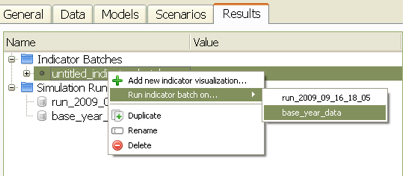
\includegraphics[width=.8\textwidth]{part-gui/images/result-manager-uncertainty1.png}
\end{center}
\caption{The ``Run Indicator Batch'' window}
\label{fig:results-manager-uncertainty1}
\end{figure}


\begin{figure}[htp]
\begin{center}
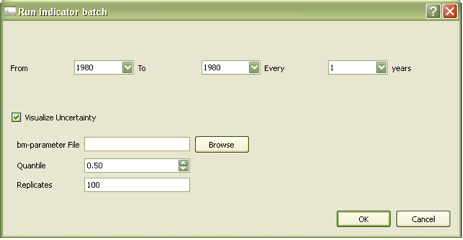
\includegraphics[width=.8\textwidth]{part-gui/images/result-manager-uncertainty2.png}
\end{center}
\caption{Checking the ``Visualize Uncertainty'' box}
\label{fig:results-manager-uncertainty2}
\end{figure}

A {\bf bm-parameter file} is used to specify bias and variance value for a
certain indicator. You must provide a bm-parameter file that has the
following structure:

{\bf first line}: base_year calibration_year \\
{\bf 2 lines per variable}: \\
\hspace*{1cm} 1. variable_name \\
\hspace*{1cm} 2. bias variance

Here is an example:
\begin{verbatim}
1979 1980
urbansim_parcel.zone.number_of_jobs
100 1000
urbansim.gridcell.population_density
7 14
urbansim.gridcell.population
5 14
\end{verbatim}

{\bf Quantile} ranges from 0.01 to 1.00. It has a default value of
0.50, which will generate a map that shows the median. Changing the
quantile value will give you the lower or upper bound for a different
confidence interval. For example, if you wish to see the lower bound
for a Confidence Interval of 90\%, since $(1-0.9)/2 = 0.05$, $0.05$ is
the quantile value that should be entered.  This means that 90\% of
the time, the values indicated on the map will be the lowest possible
values.

{\bf Replicates} has a default value of 100. When a bm-parameter file
is given, an array of size replicate is generated. Replicate value
increases accuracy.

